%!TEX root = thesis.tex

%
%==========================================================================================
%
\chapter{A Unified Detection Framework}
\label{chap:framework}

In this chapter, a unified framework for anomalous and suspicious behavior detection is presented. The goal is to design a framework rich enough to address various domains and different configurations. Therefore, we summarize its components and explain their relationships. The next part of the thesis then shows how to instantiate the detection framework in various real-life domains.

\section{Framework Components}

\index{unified framework}
All the components presented in the previous chapters form the unified framework for anomalous and suspicious behavior detection. This section reviews the components, their hierarchical structure, and explains the processing steps of the unified framework.

\subsection{Framework Levels}

Let us revisit the framework level hierarchy shown in Figure~\ref{fig:stack} that systematically processes agent spatio-temporal data to perform deviant behavior detection. The information flow is bottom-up through three main levels shown on the left-hand side: measurements, activity assessment, and behavior assessment. Each of the main levels contains several sub-levels (right-hand side): 13 in total. 

The measurement level provides sensor data, which are collected at each time step~$t$ in the next sub-level as an \emph{observation vector} $\mathbf{x}_t$. In addition to the sensor data, the observation vector may also contain contextual information and environmental variables such as time, date, weather, etc. Subsequent observation vectors are bundled in an observation sequence $\mathbf{X}$.

\index{activity recognition pipeline}
The next main level is activity assessment. The first four sub-levels basically correspond to ARPipe (activity recognition pipeline, Chapter~\ref{chap:activity_recognition}), which first suppresses the sensor noise, followed by the construction of activity recognition feature vectors and atomic activity recognition itself. Finally, the spurious transitions among atomic activities that cannot occur in reality are smoothed. \emph{Activity sequence} containing an atomic action at each time step $\avec{T}=\{a_t|1 \leq t \leq T\}$ is passed to the next sub-level, which can recognize complex behaviors or interactions among agents.

The top level performs behavior assessment in order to detect deviance. The first sub-level constructs a \emph{behavior trace} that consists of $\tuple{landmark, activity}$ tuples, which are encoded as a \emph{behavior pattern} in the next sub-level. The next sub-level then introduces a set of detectors based on different features, views and modalities to provide different evaluations of the behavior pattern. The evaluations are then combined at each time step in the next sub-level as well as over time at the level above. Finally, the top sub-level outputs the final agent behavior evaluation that comprehends all the behavior to the current time step. 

%This dissertation designs and implements a general framework for deviant behavior detection that addresses several challenges in physical domains. Within the framework four steps are introduced as shown in Figure 1: (i) activity recognition (yellow box), (ii) behavior signatures (green boxes), which are part of (iii) multi-view evaluation (blue box), and (iv) repetitive behavior detection (orange box). Each step conta


\begin{figure}[!h]
\centering
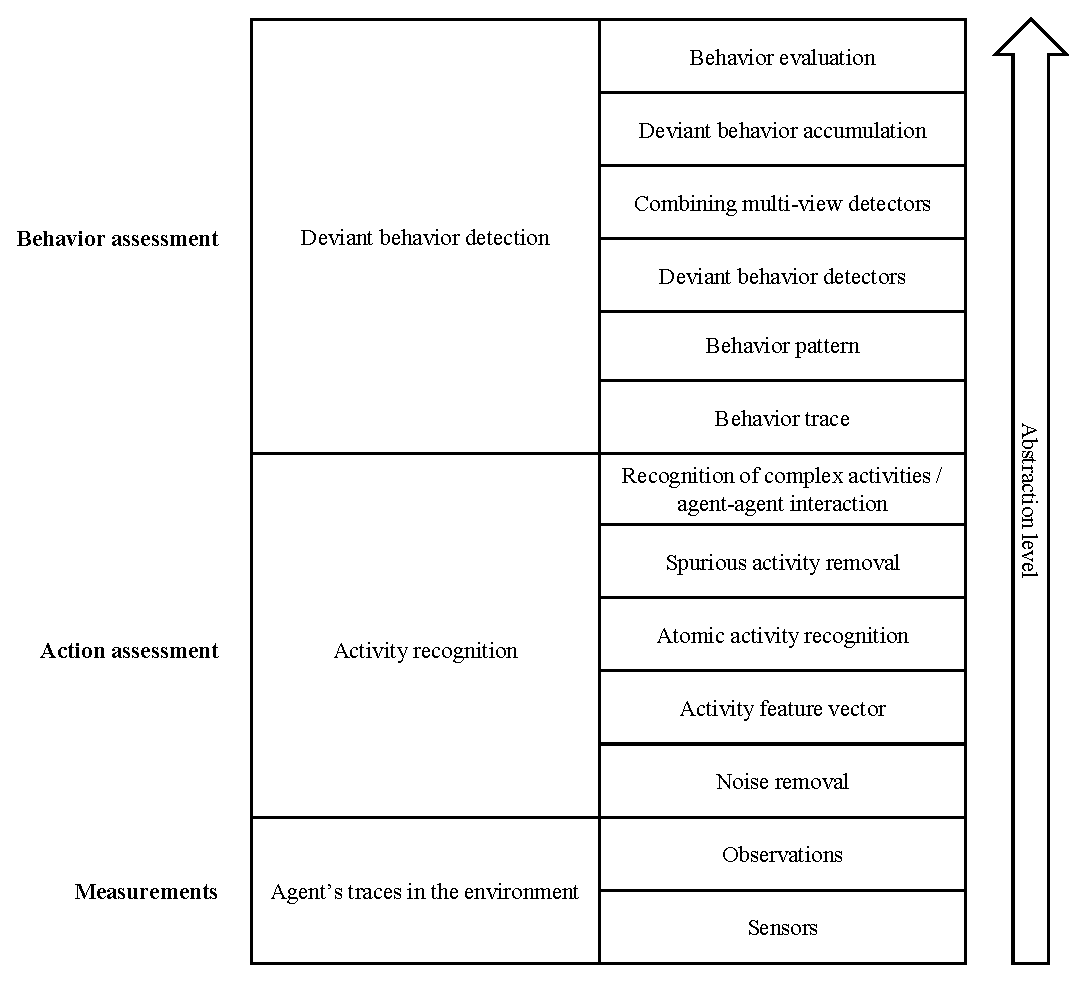
\includegraphics[width=1\textwidth]{chap_FMW/stack}
\caption{Hierarchy of abstraction levels and processes.}
\label{fig:stack}
\end{figure}

\subsection{Processing Steps}

A detailed unified framework flowchart is outlined in Figure~\ref{fig:flowchart}. The start and the end of the process are shown in rounded rectangles, processes are represented as rectangles, and input/output data are represented as a parallelogram.

The process starts with an observation sequence describing agent movements in the environment. The trace is first processed by the activity recognition pipeline as described above and outputs an activity sequence. The activity sequence then enters deviant behavior detection level marked with dashed-squared box. The activity sequence is first augmented to behavior trace, which then enters into a variety of view transformation processes. Each view-transformation process applies its specific viewpoint using either different features, modalities, or time aggregation periods to construct corresponding behavior signatures. Each behavior signature is then evaluated with a deviant behavior detector separately. The next step combines all the evaluations that are further processed in a suspicious behavior accumulation module over time, which finally outputs the input trace deviation.

General implementation principles and the theoretical background of particular flowchart processes were discussed in the previous chapters, while the concreted domain implementation is demonstrated in Part~\ref{part:applications} of this thesis. Note that, in some domains, not all the processes are required; a domain problem may simplify a certain process. For example, if only a single behavior view is required, the multi-view detector combination is simplified accordingly.

\begin{figure}[!h]
\centering
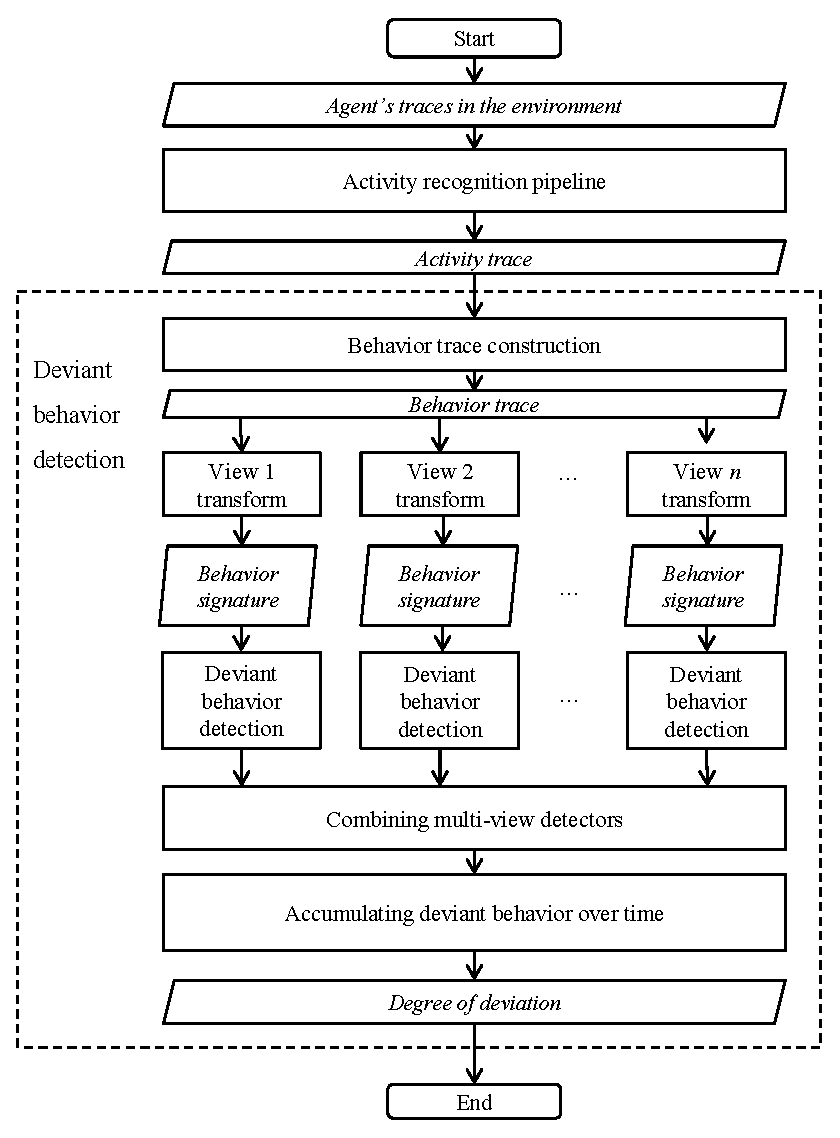
\includegraphics[width=0.8\textwidth]{chap_FMW/flowchart}
\caption{Processing flowchart of the unified framework.}
\label{fig:flowchart}
\end{figure}



\section{Framework Instantiation}
As will be shown in the next part of the thesis, the framework can be instantiated for various domains and problems. 
%The general architecture as shown in Figure~\ref{fig:stack} covers all abstraction hierarchy levels, while specific domains may omit some of the levels due to simplicity or trivial implementation. 
This section covers high-level framework instantiation, emphasizing the learning and detection phases. 

\subsection{Learning and Detection}
Unified framework instantiation includes selecting and designing some
domain-specific components as well as implementing general components described in the previous chapters. Since this will be covered in Part~\ref{part:applications} of this thesis, these components will be abstracted and the focus will be on the learning and detection phase.

Figure~\ref{fig:learning-detection} depicts a high-level block diagram of the learning (left-hand side) and the detection (right-hand side) phase within the unified framework. The goal of the learning phase is to instantiate all the components, which includes building classifiers and detectors, discovering patterns, and fine-tuning the parameters of the models. After that, the framework is deployed in the detection phase, which is dedicated to evaluating new traces at the input.

\begin{figure}[!h]
\centering
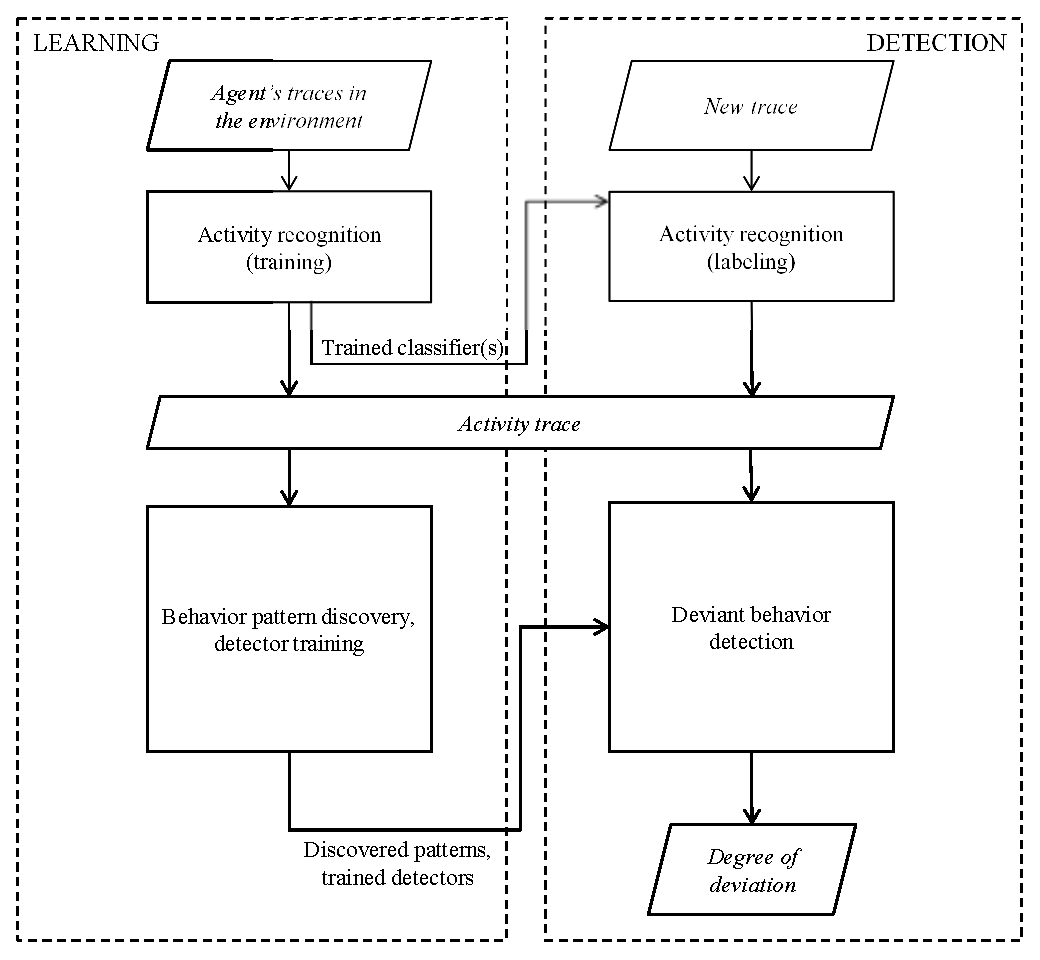
\includegraphics[width=1\textwidth]{chap_FMW/learning-detection}
\caption{Block diagram for learning and detection phases.}
\label{fig:learning-detection}
\end{figure}

The learning phase includes two components that require training. The first component is activity recognition, which, unless the activities are already provided from the environment, requires classifier training. This includes recording labeled training data to construct a training dataset, feature extraction, and building a classification model. Once the model is trained, it can be used in the detection phase. 

%implemented with expert knowledge, ... requires training data ... prerecorded activities .... feature extraction ... model selection ...

The second component is dedicated to behavior patterns construction and detection model training. According to our detection goals, that is, either anomalous or suspicious behavior detection, the aim of this phase is to construct a dataset of positive or negative behavior patterns, respectively, using either automatic/semi-automatic approaches, such as clustering, or domain expert knowledge that encodes behavior patterns. As shown in Figure~\ref{fig:flowchart}, this can be applied for a variety of viewpoints. The next step then includes detector training and initial parameter tuning, which also requires a training dataset.
Note that the second component already requires that the activity recognition component is trained.

\section{Summary}
In summary, we proposed a unified framework for detection of anomalous and suspicious behavior that can be observed from complex, spatio-temporal sequential data generated by an agent moving in a physical environment. The framework incorporates the components introduced in the previous chapters to address the main challenges. The second part of the thesis shows how the framework is instantiated in three empirical studies. 

%For example, behavior evaluation in ambient assisted living domain, where the goal is  some of the levels can be  can be 

%The framework can be applied to 

% \subsection{Framework Evaluation}

% by components...

% "celoten" performance

%\section{Discussion}
%The amount of training data